% Provenance (never printed): see sources/outline_sources.md (Year 2: humidity variables;
% Clausius--Clapeyron applied; dry and moist adiabats; thermodynamic diagrams; convective
% instability; cloud microphysics). Definitions after the NWS glossary; skew-T lines, CAPE classes
% and the lifted index after the NWS Houston/Galveston training page; saturation data from the
% NIST WebBook (IAPWS-95) and IAPWS R14-08; the empirical formula as used by Su and others
% (2026); kappa-Koehler theory after Petters and Kreidenweis (2007); CCN numbers after Andreae
% (2009); the processes of microphysics after Morrison and others (2020). The sounding is the
% real 12 UTC sounding of Norman, Oklahoma, 16 April 2026 (IGRA2); every curve and number from
% figdata/bachelor-2/thermo.py; exercise and problem values in the Book 4 scratch calculator
% calc/ch21.py.
\chapter{Thermodynamique de l'atmosphère}\label{ch:b2:atmospheric-thermodynamics}

Le 16 avril 2026, à 12~UTC, un ballon s'est élevé de la station météorologique de Norman, Oklahoma, comme des
ballons s'élèvent chaque jour à cette heure depuis plus de huit cents stations. L'instrument qu'il emportait a
renvoyé par radio un profil vertical que le prévisionniste lit d'un coup d'œil~: un air presque saturé près du
sol, un couvercle chaud et mince à six cents mètres d'altitude, et au-dessus une température qui chute vite
sur dix kilomètres. Soulevé à travers ce couvercle, l'air de surface se serait retrouvé plus chaud que son
environnement sur la plus grande partie de la troposphère, avec environ deux mille joules par kilogramme à dépenser
pour monter. Ce chapitre apprend à lire cette énergie sur un \omterm{def:b2:atmospheric-thermodynamics:sounding}{radiosondage}~: quelle quantité d'eau l'air peut
contenir, comment une particule d'air qui monte se refroidit avant et après sa condensation, comment les
diagrammes des météorologues transforment des aires en énergies, et comment les gouttelettes de nuage se forment.
% ledger: data:b4-sounding, nws4:upperair, nws4:cape

\begin{recall}
\textbf{Des volumes de physique~:} \omterm{def:b2:atmospheric-thermodynamics:moist-air}{pression de vapeur} saturante, humidité relative, point de rosée,
chaleur latente, relation de Clausius--Clapeyron et sa forme intégrée~; germination et surfusion~;
premier principe, transformations adiabatiques et capacités thermiques d'un gaz parfait.
\textbf{Des volumes de chimie~:} pressions partielles, loi de Raoult, tension superficielle et équation
de Kelvin. \textbf{Des volumes scolaires~:} le \omterm{def:b2:atmospheric-thermodynamics:lcl}{niveau de condensation} et sa règle de \qty{125}{m}
par degré, air stable et instable, le \omterm{def:b2:atmospheric-thermodynamics:microphysics}{noyau de condensation}, les processus de pluie chaude et de
cristaux de glace. \textbf{Du volume de première année~:} l'atmosphère standard, les gradients
adiabatiques de l'environnement et sec ($\Gamma_d = \qty{9.8}{K/km}$), la particule d'air, la température
potentielle, la stabilité statique, les inversions de température et l'équation hypsométrique.
\end{recall}

Dans tout le chapitre~: $R_d = R/M_d = \qty{287.0}{J.kg^{-1}.K^{-1}}$ pour l'air sec de masse
molaire \qty{28.97}{g/mol}~; $R_v = R/M_w = \qty{461.5}{J.kg^{-1}.K^{-1}}$ pour la vapeur d'eau,
de masse molaire \qty{18.0153}{g/mol}~; $\varepsilon = M_w/M_d = 0.622$~; $c_p = \tfrac72 R_d =
\qty{1004.5}{J.kg^{-1}.K^{-1}}$ (le volume de première année, avec le rapport
des capacités thermiques 1.4)~; $g = \qty{9.81}{m.s^{-2}}$~; et la
chaleur latente de vaporisation au point triple, $L = \qty{2.501e6}{J/kg}$.
% ledger: const:R, earth:Mmol, nist4:water-mw, nasa:grc-gamma, const:gn, nist4:water-sat

\section{Air humide}\label{sec:b2:atmospheric-thermodynamics:moist-air}

L'air est un mélange d'air sec et de vapeur d'eau, tous deux proches de gaz parfaits. Les
volumes de physique mesurent son eau par l'humidité relative et le point de rosée~; une
particule d'air qui monte a besoin de mesures qui ne changent pas quand elle se dilate.

\begin{definition}[Pression de vapeur~; rapport de mélange~; humidité spécifique]\label{def:b2:atmospheric-thermodynamics:moist-air}
La \emph{pression de vapeur}\index{pression de vapeur} $e$ de l'air humide est la pression
partielle de sa vapeur d'eau. Son \emph{rapport de mélange}\index{rapport de mélange} est $r = m_v/m_d$,
la masse de vapeur d'eau par unité de masse d'air sec dans le même volume, et son
\emph{humidité spécifique}\index{humidité spécifique} est $q = m_v/(m_d + m_v)$, la masse de vapeur
par unité de masse d'air humide. Les deux s'expriment d'ordinaire en grammes par kilogramme.
\end{definition}
% ledger: nws4:humidity

\begin{proposition}[Variables d'humidité]\label{prop:b2:atmospheric-thermodynamics:humidity}
Dans l'air humide à la pression totale $p$ avec la \omterm{def:b2:atmospheric-thermodynamics:moist-air}{pression de vapeur} $e$,
\[
  r = \frac{\varepsilon e}{p - e}, \qquad q = \frac{r}{1 + r} = \frac{\varepsilon e}{p - (1 -
  \varepsilon)e} .
\]
À saturation, $e = e_s(T)$ et $r = r_s(T, p)$, le \omterm{def:b2:atmospheric-thermodynamics:moist-air}{rapport de mélange} de saturation. Ni $r$ ni
$q$ ne changent lorsqu'une particule se dilate ou se comprime sans gagner ni perdre d'eau.
\end{proposition}

\begin{proof}
Dans le même volume $V$ à la température $T$, chaque gaz obéit à sa propre loi des gaz
parfaits avec sa pression partielle~: $m_v = eV/(R_vT)$ et $m_d = (p - e)V/(R_dT)$, donc
$r = (R_d/R_v)\,e/(p - e)$, et $R_d/R_v = M_w/M_d = \varepsilon$. Diviser $m_v$ par $m_d + m_v$
donne $q = r/(1 + r)$. La dilatation change $V$, $p$ et $e$, mais pas les deux masses.
\end{proof}

\begin{definition}[Température virtuelle]\label{def:b2:atmospheric-thermodynamics:virtual}
La \emph{température virtuelle}\index{température virtuelle} $T_v$ de l'air humide est la
température que l'air sec devrait avoir, à même pression, pour avoir la même masse volumique~:
\[
  T_v = T\,\frac{1 + r/\varepsilon}{1 + r} \approx T\,(1 + 0.61\,r) .
\]
\end{definition}
% ledger: nws4:virtual-theta-e

La démonstration que cette température tient ce qu'elle promet tient en une ligne~: la masse volumique
de l'air humide vaut $(m_d + m_v)/V = \bigl(p - e\bigr)/(R_dT) + e/(R_vT)$, qui, avec
$e = pr/(\varepsilon + r)$, vaut $p/(R_dT_v)$. La vapeur d'eau est plus légère que l'air sec~: l'air humide est donc
moins dense que l'air sec à même température et même pression, comme s'il était un peu plus chaud.

\begin{example}[L'air de Norman]\label{ex:b2:atmospheric-thermodynamics:norman}
Au sol, le \omterm{def:b2:atmospheric-thermodynamics:sounding}{radiosondage} donne $p = \qty{971.1}{hPa}$, $T = \qty{19.0}{\celsius}$ et un point
de rosée de \qty{18.5}{\celsius}. La \omterm{def:b2:atmospheric-thermodynamics:moist-air}{pression de vapeur} est la \omterm{def:b2:atmospheric-thermodynamics:moist-air}{pression de vapeur} saturante
au point de rosée, $e = e_s(\qty{18.5}{\celsius}) = \qty{21.5}{hPa}$
(\cref{prop:b2:atmospheric-thermodynamics:es} ci-dessous). Alors $r = 0.622 \times 21.5/(971.1 - 21.5) = \qty{14.1}{g/kg}$,
$q = \qty{13.9}{g/kg}$, et $T_v - T = 0.61 \times 0.0141 \times \qty{292.15}{K} = \qty{2.5}{K}$~:
cet air est aussi léger que de l'air sec deux degrés et demi plus chaud.
\end{example}
% ledger: data:b4-sounding

\section{Pression de vapeur saturante}\label{sec:b2:atmospheric-thermodynamics:saturation}

Au-dessus d'une surface plane d'eau pure, la \omterm{def:b2:atmospheric-thermodynamics:moist-air}{pression de vapeur} à l'équilibre ne dépend que
de la température. Les volumes de physique en établissent la loi, la relation de Clausius--Clapeyron,
et l'intègrent à chaleur latente constante~; pour la vapeur d'eau, $M L/R = L/R_v$.

\begin{proposition}[Pression de vapeur saturante]\label{prop:b2:atmospheric-thermodynamics:es}
La chaleur latente $L$ étant supposée constante, la \omterm{def:b2:atmospheric-thermodynamics:moist-air}{pression de vapeur} saturante au-dessus de l'eau est
\[
  e_s(T) = e_t \exp\!\Bigl[\frac{L}{R_v}\Bigl(\frac{1}{T_t} - \frac{1}{T}\Bigr)\Bigr],
  \qquad e_t = \qty{6.117}{hPa}, \quad T_t = \qty{273.16}{K}, \quad \frac{L}{R_v} =
  \qty{5419}{K},
\]
où $(T_t, e_t)$ est le point triple de l'eau.
\end{proposition}
% ledger: iapws4:sublimation, nist4:water-sat

\begin{corollary}[Sept pour cent par kelvin]\label{cor:b2:atmospheric-thermodynamics:seven}
Le taux relatif d'accroissement de la \omterm{def:b2:atmospheric-thermodynamics:moist-air}{pression de vapeur} saturante
est $\mathrm{d}\ln e_s/\mathrm{d}T = L/(R_v T^2)$~:
\qty{7.3}{\percent} par kelvin à \qty{0}{\celsius}, \qty{6.3}{\percent}
à \qty{20}{\celsius}, \qty{5.9}{\percent} à \qty{30}{\celsius}.
\end{corollary}

La chaleur latente constante est le seul défaut de la formule~: la chaleur latente passe de
\qty{2500.9}{kJ/kg} au point triple à \qty{2453.5}{kJ/kg} à \qty{20}{\celsius}, si bien que la
formule dépasse les valeurs mesurées à mesure que la température s'élève, de \qty{1.2}{\percent} à
\qty{20}{\celsius} et de \qty{2.5}{\percent} à \qty{30}{\celsius} (figure ci-dessous). Une
formule empirique ajustée sur des mesures, $e_s = \qty{6.112}{hPa} \times \exp[17.67\,t/(t + 243.5)]$
avec $t$ en degrés Celsius, reste à quelques pour mille près~; les produits de données
l'utilisent, mais la proposition est celle qui se dérive et se comprend, et ce chapitre la garde.
% ledger: nist4:water-sat, su26:svp

Au-dessous de \qty{0}{\celsius}, l'eau peut rester liquide dans les nuages, en surfusion, et il
existe deux \omterm{def:b2:atmospheric-thermodynamics:moist-air}{pressions de vapeur} saturante~: au-dessus de l'eau liquide et au-dessus de la glace.
La seconde est plus basse, car la chaleur latente de sublimation dépasse celle de vaporisation
d'une quantité égale à la chaleur latente de fusion. L'air saturé par rapport aux gouttelettes
en surfusion est sursaturé par rapport à la glace, de \qty{10}{\percent} à \qty{-10}{\celsius}
et de \qty{22}{\percent} à \qty{-20}{\celsius}~: la dernière section revient sur cet écart.
% ledger: iapws4:sublimation, su26:svp

\begin{omfigure}
\centering
% figdata/bachelor-2/thermo.py parts es, nist
\begin{tikzpicture}
\begin{groupplot}[group style={group size=2 by 1, horizontal sep=1.9cm},
  width=0.44\linewidth, height=5.4cm, tick label style={font=\scriptsize},
  label style={font=\small}]
\nextgroupplot[xmin=-40, xmax=40, ymin=0, ymax=80, xlabel={température (\unit{\celsius})},
  ylabel={pression de vapeur saturante (\unit{hPa})}, legend pos=north west,
  legend style={font=\scriptsize, draw=none, fill=none}, legend cell align=left]
\addplot[ocBlue, thick] table[x=T_C, y=cc] {figdata/out/bachelor-2-thermo-es.dat};
\addlegendentry{relation théorique}
\addplot[black, densely dashed] table[x=T_C, y=emp] {figdata/out/bachelor-2-thermo-es.dat};
\addlegendentry{formule empirique}
\addplot[only marks, mark=*, mark size=1.4pt, ocRed] table[x=T_C, y=es_hPa]
  {figdata/out/bachelor-2-thermo-nist.dat};
\addlegendentry{mesurée (IAPWS-95)}
\nextgroupplot[xmin=-40, xmax=0, ymin=1, ymax=1.5, xlabel={température (\unit{\celsius})},
  ylabel={$e_s(\text{eau})/e_s(\text{glace})$}]
\addplot[omMeth, thick, unbounded coords=discard] table[x=T_C, y=wi]
  {figdata/out/bachelor-2-thermo-es.dat};
\draw[black!40, densely dotted] (axis cs:-10,1) -- (axis cs:-10,1.1035) -- (axis cs:-40,1.1035);
\node[font=\scriptsize, anchor=south west] at (axis cs:-10,1.1035) {1.10};
\draw[black!40, densely dotted] (axis cs:-20,1) -- (axis cs:-20,1.218) -- (axis cs:-40,1.218);
\node[font=\scriptsize, anchor=south west] at (axis cs:-20,1.218) {1.22};
\end{groupplot}
\end{tikzpicture}
\par\smallskip{\small À gauche~: la \omterm{def:b2:atmospheric-thermodynamics:moist-air}{pression de vapeur} saturante au-dessus de l'eau, selon la
\cref{prop:b2:atmospheric-thermodynamics:es}, selon la formule empirique et telle que mesurée. À droite~: le rapport des
\omterm{def:b2:atmospheric-thermodynamics:moist-air}{pressions de vapeur} saturante au-dessus de l'eau en surfusion (formule empirique) et au-dessus de la
glace (équation de sublimation de l'IAPWS).}
\end{omfigure}
% ledger: nist4:water-sat, iapws4:sublimation, su26:svp

\section{Ascension de l'air humide}\label{sec:b2:atmospheric-thermodynamics:ascent}

Une particule qui monte sans échanger de chaleur se refroidit au gradient adiabatique sec, conserve sa
température potentielle et, si elle ne condense pas, conserve son \omterm{def:b2:atmospheric-thermodynamics:moist-air}{rapport de mélange}. Sa \omterm{def:b2:atmospheric-thermodynamics:moist-air}{pression de vapeur}
$e = pr/(\varepsilon + r)$ baisse avec la pression, mais sa \omterm{def:b2:atmospheric-thermodynamics:moist-air}{pression de vapeur} saturante baisse plus vite,
avec sa température. Les deux se rejoignent à un niveau que les volumes scolaires trouvent par une règle.

\begin{definition}[Niveau de condensation par soulèvement]\label{def:b2:atmospheric-thermodynamics:lcl}
Le \emph{niveau de condensation par soulèvement}\index{niveau de condensation par soulèvement}
(LCL) d'une particule d'air est le niveau où elle devient saturée lorsqu'elle est soulevée de
façon adiabatique sèche. C'est le \emph{niveau de condensation}\index{niveau de condensation}
des volumes scolaires, la hauteur des bases planes des nuages qui se forment par soulèvement.
\end{definition}
% ledger: nws4:lcl

\begin{proposition}[Hauteur du niveau de condensation par soulèvement]\label{prop:b2:atmospheric-thermodynamics:lcl}
Une particule à la température $T$ de point de rosée $T_d$ atteint la saturation environ
\[
  z_{\text{LCL}} \approx \frac{T - T_d}{\Gamma_d - \Gamma_{\text{rosée}}}, \qquad
  \Gamma_{\text{rosée}} = \frac{g R_v T_d^2}{L R_d T} \approx \qty{1.8}{K/km},
\]
au-dessus de son niveau de départ~: environ \qty{125}{m} par degré de dépression du point de rosée.
\end{proposition}

\begin{proof}
La température de la particule baisse au taux $\Gamma_d$. Son point de rosée est la température
à laquelle sa \omterm{def:b2:atmospheric-thermodynamics:moist-air}{pression de vapeur} $e$ atteindrait la saturation~; à $r$ constant, $e$ est
proportionnelle à $p$, donc $\mathrm{d}\ln e = \mathrm{d}\ln p = -g\,\mathrm{d}z/(R_dT)$ par l'équilibre
hydrostatique. D'après la \cref{prop:b2:atmospheric-thermodynamics:es},
$\mathrm{d}\ln e = L\,\mathrm{d}T_d/(R_vT_d^2)$. D'où $\mathrm{d}T_d/\mathrm{d}z = -gR_vT_d^2/(LR_dT) = -\Gamma_{\text{rosée}}$~:
le point de rosée baisse aussi, mais plus lentement. L'écart $T - T_d$ se referme
au taux $\Gamma_d - \Gamma_{\text{rosée}}$. Avec $T \approx T_d \approx \qty{288}{K}$,
$\Gamma_{\text{rosée}} = \qty{1.8}{K/km}$, et $1/(9.8 - 1.8)$ kilomètre par kelvin fait \qty{125}{m}.
\end{proof}

À Norman, la dépression du point de rosée était de \qty{0.5}{K}~: l'air de surface aurait
condensé après \qty{63}{m} de montée, à \qty{964}{hPa}. Le calcul complet, qui suit
l'adiabatique sèche et le \omterm{def:b2:atmospheric-thermodynamics:moist-air}{rapport de mélange} de saturation sans linéariser, donne \qty{64}{m}.
% ledger: data:b4-sounding

Au-dessus du LCL, la particule condense en montant. La condensation libère
de la chaleur latente, et la particule se refroidit plus lentement.

\begin{definition}[Gradient adiabatique saturé~; adiabatique humide]\label{def:b2:atmospheric-thermodynamics:moist-adiabat}
Le \emph{gradient adiabatique saturé}\index{gradient adiabatique saturé} $\Gamma_s$
est le taux auquel baisse la température d'une particule saturée qui monte, sa vapeur
condensant pour la maintenir saturée. La courbe qu'elle suit sur un diagramme
température-pression est une \emph{adiabatique humide}\index{adiabatique humide}. Lorsque
l'eau condensée est supposée retomber aussitôt, la montée est dite pseudo-adiabatique.
\end{definition}
% ledger: nws4:malr

\begin{proposition}[Gradient adiabatique saturé]\label{prop:b2:atmospheric-thermodynamics:gamma-s}
Pour une montée pseudo-adiabatique, avec $r_s = r_s(T, p)$,
\[
  \Gamma_s = g\,\frac{1 + \dfrac{L r_s}{R_d T}}{c_p + \dfrac{L^2 r_s}{R_v T^2}} .
\]
Il tend vers $\Gamma_d = g/c_p$ lorsque $r_s$ tend vers zéro, et il est plus petit sinon.
\end{proposition}

\begin{proof}
Par unité de masse d'air sec, le premier principe pour une particule qui reçoit la chaleur latente de la
vapeur qu'elle condense, $-L\,\mathrm{d}r_s$, s'écrit $c_p\,\mathrm{d}T - (R_dT/p)\,\mathrm{d}p = -L\,
\mathrm{d}r_s$~; avec l'équilibre hydrostatique $(R_dT/p)\,\mathrm{d}p = -g\,\mathrm{d}z$, il devient
$c_p\,\mathrm{d}T + g\,\mathrm{d}z + L\,\mathrm{d}r_s = 0$. Avec $r_s \approx \varepsilon e_s/p$,
$\mathrm{d}r_s = r_s\,(\mathrm{d}\ln e_s - \mathrm{d}\ln p) = r_s\bigl(L\,\mathrm{d}T/(R_vT^2) +
g\,\mathrm{d}z/(R_dT)\bigr)$. En substituant et en regroupant les termes en
$\mathrm{d}T$ et en $\mathrm{d}z$, on obtient $-\mathrm{d}T/\mathrm{d}z = \Gamma_s$.
\end{proof}

Le taux dépend de la quantité d'eau à condenser. À \qty{1000}{hPa}, il vaut \qty{6.5}{K/km} à
\qty{0}{\celsius}, \qty{5.2}{K/km} à \qty{10}{\celsius}, \qty{4.2}{K/km} à \qty{20}{\celsius}
et \qty{3.4}{K/km} à \qty{30}{\celsius}~; haut dans la troposphère, à \qty{200}{hPa} et
\qty{-60}{\celsius}, il revient à \qty{9.6}{K/km}, presque le taux sec. Une \omterm{def:b2:atmospheric-thermodynamics:moist-adiabat}{adiabatique humide}
est donc raide près d'un sol chaud et s'infléchit vers les adiabatiques sèches en altitude.
% ledger: nws4:malr

\begin{definition}[Température potentielle équivalente]\label{def:b2:atmospheric-thermodynamics:theta-e}
La \emph{température potentielle équivalente}\index{température potentielle équivalente} $\theta_e$ d'une particule
est la température qu'elle aurait si on la soulevait jusqu'à ce que toute sa vapeur ait condensé et soit
retombée, puis si on la ramenait de façon adiabatique sèche jusqu'à \qty{1000}{hPa}. Une bonne approximation est
\[
  \theta_e \approx \theta \exp\!\Bigl(\frac{L r}{c_p T_{\text{LCL}}}\Bigr),
\]
avec $\theta$ la température potentielle et $T_{\text{LCL}}$ la
température au \omterm{def:b2:atmospheric-thermodynamics:lcl}{niveau de condensation par soulèvement} de la particule.
\end{definition}
% ledger: nws4:virtual-theta-e

La température potentielle n'est conservée que dans une montée sèche~; $\theta_e$ est conservée, à cette approximation,
dans une montée sèche comme saturée, car la chaleur qu'elle compte comme déjà libérée est exactement celle
que libère la condensation. Elle désigne une \omterm{def:b2:atmospheric-thermodynamics:moist-adiabat}{adiabatique humide} comme $\theta$ désigne une adiabatique sèche.
L'air de surface de Norman a $\theta = 292.15 \times (1000/971.1)^{2/7} = \qty{294.6}{K}$ et
$\theta_e = 294.6 \exp[2.501 \times 10^6 \times 0.0141/(1004.5 \times 291.5)] = \qty{332}{K}$.
% ledger: data:b4-sounding

\section{Diagrammes thermodynamiques}\label{sec:b2:atmospheric-thermodynamics:diagrams}

\begin{definition}[Radiosondage]\label{def:b2:atmospheric-thermodynamics:sounding}
Un \emph{radiosondage}\index{radiosondage} est un profil vertical de la pression, de
la température, de l'humidité et du vent de l'atmosphère au-dessus d'un lieu, mesuré
par un instrument emporté en altitude, le plus souvent une radiosonde sous un ballon.
\end{definition}
% ledger: nws:radiosonde, nws4:upperair

Un \omterm{def:b2:atmospheric-thermodynamics:sounding}{radiosondage} n'est ni tout à fait vertical, car le ballon dérive avec le vent, ni tout à
fait instantané, car il lui faut plusieurs minutes pour atteindre la haute troposphère~; le
réseau principal ne lâche des ballons que deux fois par jour. Ses nombres deviennent utiles une
fois portés sur un diagramme où une particule d'air qui monte peut être suivie à la règle.
% ledger: hgx:skewt-lines

\begin{definition}[Diagramme thermodynamique~; émagramme oblique (skew-T log-p)~; téphigramme]\label{def:b2:atmospheric-thermodynamics:diagram}
Un \emph{diagramme thermodynamique}\index{diagramme thermodynamique} est un graphique dont les coordonnées
sont des fonctions de la pression et de la température, sur lequel sont tracés les isobares, les
isothermes, les adiabatiques sèches, les \omterm{def:b2:atmospheric-thermodynamics:moist-adiabat}{adiabatiques humides} et les lignes de \omterm{def:b2:atmospheric-thermodynamics:moist-air}{rapport de mélange} de
saturation constant, et sur lequel un \omterm{def:b2:atmospheric-thermodynamics:sounding}{radiosondage} est porté sous forme de deux courbes, sa température
et son point de rosée. Sur un \emph{émagramme oblique}\index{émagramme oblique} (skew-T log-p), la
coordonnée verticale est $-\ln p$ et l'horizontale est $T + k\ln(p_0/p)$, de sorte que les isobares sont
horizontales et que les isothermes sont des droites obliques montant vers la droite. Un
\emph{téphigramme}\index{téphigramme} utilise pour coordonnées la température et l'entropie par unité de masse
$c_p\ln\theta$, de sorte que les isothermes et les adiabatiques sèches sont des droites perpendiculaires.
\end{definition}
% ledger: hgx:skewt-lines

\begin{proposition}[Les aires sont des énergies]\label{prop:b2:atmospheric-thermodynamics:areas}
Sur un \omterm{def:b2:atmospheric-thermodynamics:diagram}{émagramme oblique} (skew-T log-p), l'aire comprise entre deux courbes $T_1(p)$ et $T_2(p)$
entre les pressions $p_b > p_a$ est proportionnelle à $\int_{p_a}^{p_b} R_d\,(T_1 - T_2)\,\mathrm{d}\ln p$,
l'énergie par unité de masse que la \cref{prop:b2:atmospheric-thermodynamics:buoyancy}
ci-dessous donne à une particule suivant $T_1$ à travers un environnement $T_2$.
\end{proposition}

\begin{proof}
Prenons $Y = \ln(p_0/p)$ et $X = T + kY$. Le jacobien de $(T, Y) \mapsto (X, Y)$ vaut 1, donc les aires
dans le plan $(X, Y)$ sont égales aux aires dans le plan $(T, Y)$, où l'aire comprise entre deux
courbes vaut $\int (T_1 - T_2)\,\mathrm{d}Y = \int (T_1 - T_2)\,\mathrm{d}\ln p$, prise de $p_a$ à $p_b$
avec le signe fixé. En multipliant par $R_d$ et par l'échelle du diagramme, on obtient l'énergie.
\end{proof}

\begin{method}[Soulever une particule sur un diagramme]\label{met:b2:atmospheric-thermodynamics:lift}
\begin{enumerate}
  \item Tracer la température et le point de rosée du \omterm{def:b2:atmospheric-thermodynamics:sounding}{radiosondage} en fonction de la pression.
  \item Depuis la température de la particule, suivre l'adiabatique sèche vers le haut~; depuis son point de rosée,
        suivre la ligne de \omterm{def:b2:atmospheric-thermodynamics:moist-air}{rapport de mélange} de saturation. Leur point de rencontre est le LCL.
  \item Depuis le LCL, suivre l'\omterm{def:b2:atmospheric-thermodynamics:moist-adiabat}{adiabatique humide} vers le haut.
  \item Là où la courbe de la particule se trouve à droite de la température du \omterm{def:b2:atmospheric-thermodynamics:sounding}{radiosondage}, la
        particule est plus chaude que son environnement~; les niveaux où les deux courbes se croisent
        sont les niveaux de la \cref{def:b2:atmospheric-thermodynamics:parcel-levels} ci-dessous.
\end{enumerate}
\end{method}
% ledger: hgx:skewt-lines


\section{Stabilité et énergie convective}\label{sec:b2:atmospheric-thermodynamics:stability}

Le volume de première année comparait le gradient vertical $\Gamma$ d'une couche à $\Gamma_d$. Une particule
saturée se refroidit à $\Gamma_s$ à la place, et un troisième cas apparaît entre les deux gradients.

\begin{definition}[Instabilité conditionnelle]\label{def:b2:atmospheric-thermodynamics:instability}
Une couche dont le gradient vertical se situe entre les \omterm{def:b2:atmospheric-thermodynamics:moist-adiabat}{gradients adiabatiques saturé} et sec,
$\Gamma_s < \Gamma < \Gamma_d$, est en \emph{instabilité conditionnelle}\index{instabilité conditionnelle}~:
stable pour les particules non saturées, instable pour les particules saturées.
\end{definition}
% ledger: nws4:malr

À Norman, la température a baissé de \qty{37.0}{K} entre \qty{850}{hPa} (\qty{1489}{m})
et \qty{500}{hPa} (\qty{5725}{m}), soit \qty{8.7}{K/km}~: \omterm{def:b2:atmospheric-thermodynamics:instability}{instabilité conditionnelle}
sur quatre kilomètres. Le déclenchement de l'instabilité dépend de l'endroit où
une particule venue d'en bas devient saturée, puis plus chaude que son environnement.
% ledger: data:b4-sounding

\begin{definition}[Niveau de convection libre~; niveau d'équilibre]\label{def:b2:atmospheric-thermodynamics:parcel-levels}
Le \emph{niveau de convection libre}\index{niveau de convection libre} (LFC) d'une particule
soulevée est le niveau au-dessus duquel, saturée, elle devient plus chaude que son
environnement et monte librement. Le \emph{niveau d'équilibre}\index{niveau d'équilibre} (EL) est
le niveau au-dessus du LFC où sa température redevient égale à celle de son environnement.
\end{definition}
% ledger: nws4:lfc-el

\begin{omfigure}
\centering
% figdata/bachelor-2/thermo.py parts iso, dry, moist, mix, env, dew, parcel, cape, cin, marks
\begin{tikzpicture}
\begin{axis}[width=0.86\linewidth, height=10.6cm, ymode=log, y dir=reverse, ymin=100,
  ymax=1050, xmin=-42, xmax=44, clip=true,
  ytick={100,200,300,400,500,700,850,1000}, yticklabels={100,200,300,400,500,700,850,1000},
  minor ytick={}, xtick={-41.464,-31.464,-21.464,-11.464,-1.464,8.536,18.536,28.536,38.536},
  xticklabels={$-40$,$-30$,$-20$,$-10$,0,10,20,30,40}, tick label style={font=\scriptsize},
  xlabel={température (\unit{\celsius}), lue le long des isothermes obliques},
  ylabel={pression (\unit{hPa})}, label style={font=\small},
  legend style={font=\scriptsize, at={(0.985,0.985)}, anchor=north east, fill=white,
  fill opacity=0.9, text opacity=1, draw=black!30}, legend cell align=left]
\addplot[fill=ocRed, fill opacity=0.28, draw=none, forget plot] table[x=x, y=p]
  {figdata/out/bachelor-2-thermo-cape.dat};
\addplot[fill=ocBlue, fill opacity=0.28, draw=none, forget plot] table[x=x, y=p]
  {figdata/out/bachelor-2-thermo-cin.dat};
\addplot[black!22, very thin, forget plot] table[x=x, y=p] {figdata/out/bachelor-2-thermo-iso.dat};
\addplot[orange!70!black, very thin, opacity=0.55] table[x=x, y=p]
  {figdata/out/bachelor-2-thermo-dry.dat};
\addlegendentry{adiabatiques sèches}
\addplot[omMeth, very thin, densely dashed, opacity=0.7] table[x=x, y=p]
  {figdata/out/bachelor-2-thermo-moist.dat};
\addlegendentry{adiabatiques humides}
\addplot[ocBlue, thin, dotted] table[x=x, y=p]
  {figdata/out/bachelor-2-thermo-mix.dat};
\addlegendentry{rapport de mélange de saturation}
\addplot[ocRed, thick] table[x=x, y=p] {figdata/out/bachelor-2-thermo-env.dat};
\addlegendentry{température}
\addplot[omMeth!70!black, thick] table[x=x, y=p] {figdata/out/bachelor-2-thermo-dew.dat};
\addlegendentry{point de rosée}
\addplot[black, thick, dashed] table[x=x, y=p] {figdata/out/bachelor-2-thermo-parcel.dat};
\addlegendentry{particule de surface}
\foreach \r/\x in {1/-7.948, 2/0.283, 4/9.053, 8/18.396, 16/28.323} {
  \edef\tmp{\noexpand\node[font=\noexpand\tiny, ocBlue, anchor=south] at (axis cs:\x,600) {\r};}\tmp
}
\addplot[only marks, mark=*, mark size=1.6pt, black, forget plot] table[x=x, y=p]
  {figdata/out/bachelor-2-thermo-marks.dat};
\node[font=\scriptsize, anchor=west] at (axis cs:20.5,963.9) {LCL};
\node[font=\scriptsize, anchor=west] at (axis cs:18.2,732.5) {LFC};
\node[font=\scriptsize, anchor=east] at (axis cs:-9.6,235.6) {EL};
\node[font=\scriptsize, ocRed!70!black] at (axis cs:2,420) {CAPE};
\node[font=\scriptsize, ocBlue!70!black, anchor=west] at (axis cs:27,860) {CIN};
\end{axis}
\end{tikzpicture}
\par\smallskip{\small Le \omterm{def:b2:atmospheric-thermodynamics:sounding}{radiosondage} de 12~UTC à Norman, Oklahoma, le 16 avril 2026, sur un \omterm{def:b2:atmospheric-thermodynamics:diagram}{émagramme
oblique} (skew-T log-p), avec la particule de surface soulevée le long de son adiabatique sèche jusqu'au LCL
puis de son \omterm{def:b2:atmospheric-thermodynamics:moist-adiabat}{adiabatique humide} au-dessus. Rouge~: l'aire positive (CAPE)~; bleu~: l'aire négative sous le LFC (CIN),
toutes deux calculées avec la température. \omterm{def:b2:atmospheric-thermodynamics:moist-air}{Rapports de mélange} de saturation en grammes par kilogramme,
indiqués à \qty{600}{hPa}.}
\end{omfigure}
% ledger: data:b4-sounding, hgx:skewt-lines

\begin{definition}[Énergie potentielle convective disponible~; inhibition convective]\label{def:b2:atmospheric-thermodynamics:cape}
L'\emph{énergie potentielle convective disponible}\index{énergie potentielle convective disponible}
(CAPE) d'une particule est le travail de la force de flottabilité sur l'unité de masse de celle-ci entre son LFC et son
EL,
\[
  \text{CAPE} = \int_{z_{\text{LFC}}}^{z_{\text{EL}}} g\,\frac{T_{v,\text{particule}} -
  T_{v,\text{milieu}}}{T_{v,\text{milieu}}}\,\mathrm{d}z ,
\]
et son \emph{inhibition convective}\index{inhibition convective} (CIN)
est la même intégrale, négative, du niveau de départ jusqu'à son LFC.
\end{definition}
% ledger: nws4:cape, nws4:cin

\begin{proposition}[Flottabilité sur un diagramme~; vitesse de la particule]\label{prop:b2:atmospheric-thermodynamics:buoyancy}
\begin{enumerate}
  \item En fonction de la pression, $\text{CAPE} = R_d \int_{p_{\text{EL}}}^{p_{\text{LFC}}}
        (T_{v,\text{particule}} - T_{v,\text{milieu}})\,\mathrm{d}\ln p$~: sur un \omterm{def:b2:atmospheric-thermodynamics:diagram}{émagramme oblique}, elle est
        proportionnelle à l'aire comprise entre la courbe de la particule et le \omterm{def:b2:atmospheric-thermodynamics:sounding}{radiosondage}.
  \item Une particule qui quitte le LFC au repos et qui conserve tout le travail de sa flottabilité
        atteint le \omterm{def:b2:atmospheric-thermodynamics:parcel-levels}{niveau d'équilibre} avec la vitesse verticale $w_{\max} = \sqrt{2\,\text{CAPE}}$.
\end{enumerate}
\end{proposition}

\begin{proof}
1. La particule et son environnement partagent la pression, donc le rapport des masses volumiques
est celui des \omterm{def:b2:atmospheric-thermodynamics:virtual}{températures virtuelles}, et la force de flottabilité par unité de masse vaut
$g(T_{v,\text{particule}} - T_{v,\text{milieu}})/T_{v,\text{milieu}}$. L'environnement est hydrostatique~:
$\mathrm{d}z = -R_dT_{v,\text{milieu}}\,\mathrm{d}\ln p/g$. En substituant, $g$ et $T_{v,\text{milieu}}$
se simplifient~; l'aire découle de la \cref{prop:b2:atmospheric-thermodynamics:areas}. 2. Avec $b$
la force de flottabilité par unité de masse, $\mathrm{d}w/\mathrm{d}t = b$ et $w = \mathrm{d}z/
\mathrm{d}t$ donnent $w\,\mathrm{d}w = b\,\mathrm{d}z$~; en intégrant depuis le
LFC, où $w = 0$, jusqu'au \omterm{def:b2:atmospheric-thermodynamics:parcel-levels}{niveau d'équilibre}, on obtient $w^2/2 = \text{CAPE}$.
\end{proof}

\begin{example}[L'énergie du radiosondage de Norman]\label{ex:b2:atmospheric-thermodynamics:cape}
Soulevons l'air de surface de l'\cref{ex:b2:atmospheric-thermodynamics:norman}. Il sature à \qty{964}{hPa},
\qty{64}{m} plus haut, et suit une \omterm{def:b2:atmospheric-thermodynamics:moist-adiabat}{adiabatique humide}. Sous \qty{900}{hPa}, le \omterm{def:b2:atmospheric-thermodynamics:sounding}{radiosondage} est
lui-même presque saturé et la particule reste quelques dixièmes de degré plus froide que son environnement~;
vient ensuite l'inversion entre \qty{908}{hPa} et \qty{889}{hPa}, où la température monte de \qty{4.1}{K}
sur \qty{178}{m} et où la particule se trouve \qty{5}{K} trop froide. Ce n'est qu'à \qty{732}{hPa},
\qty{2.4}{km} au-dessus du sol, qu'elle devient plus chaude que son environnement~: c'est son LFC~;
elle le reste jusqu'à son EL, à \qty{236}{hPa}, \qty{10.9}{km} au-dessus du niveau de la mer, juste sous
la tropopause que le \omterm{def:b2:atmospheric-thermodynamics:sounding}{radiosondage} situe à \qty{235}{hPa}. Sur une grille fine de pressions, les aires
du diagramme skew-T donnent une CAPE $= \qty{2100}{J/kg}$ et une CIN $= \qty{-200}{J/kg}$ avec la
température, et \qty{2230}{J/kg} et \qty{-130}{J/kg} avec la \omterm{def:b2:atmospheric-thermodynamics:virtual}{température virtuelle}~: l'humidité de la particule
ajoute sa propre flottabilité. La théorie de la particule donne $w_{\max} = \sqrt{2 \times 2100} =
\qty{65}{m/s}$.
\end{example}
% ledger: data:b4-sounding

Les tables des prévisionnistes déclarent positive une CAPE allant jusqu'à \qty{1500}{J/kg}, grande une CAPE comprise
entre \qty{1500}{J/kg} et \qty{2500}{J/kg}, et extrême une CAPE au-delà de \qty{2500}{J/kg}~; des valeurs supérieures
à \qty{1000}{J/kg} sont courantes dans les environnements d'orage, et les valeurs au-delà de \qty{5000}{J/kg} sont
rares. La CAPE est la plus forte en saison chaude, surtout à la fin du printemps. L'indice de soulèvement, soit la
température du \omterm{def:b2:atmospheric-thermodynamics:sounding}{radiosondage} à \qty{500}{hPa} moins celle de la particule soulevée, résume la même information en un seul
nombre~: à Norman, $-18.4 - (-8.9) = \qty{-9.5}{K}$, dans la classe de $-8$ à $-10$ que les tables des prévisionnistes
appellent instabilité extrême. Aucune de ces valeurs n'est un seuil au-delà duquel des orages doivent se former.
% ledger: hgx:cape, nws4:cape, nws4:lifted-index

La CIN est le prix à payer. Le couvercle chaud a empêché l'air de surface de monter de lui-même~: une particule
devrait être poussée au travers, par un front ou par la lente ascension de l'air situé devant une perturbation
en altitude, ou être réchauffée par le bas par le soleil de l'après-midi jusqu'à être flottante sur toute
la hauteur. Et la vitesse $w_{\max}$ est une borne supérieure~: un courant ascendant réel emporte son eau
condensée, qui l'alourdit, et se mélange à l'air plus sec qui l'entoure, lequel le refroidit par évaporation.
Le \omterm{def:b2:atmospheric-thermodynamics:parcel-levels}{niveau d'équilibre} reste un bon indicateur de l'endroit où les sommets de l'orage s'étalent en enclume.
% ledger: nws4:cin, hgx:cape, nws4:lfc-el

\begin{omfigure}
\centering
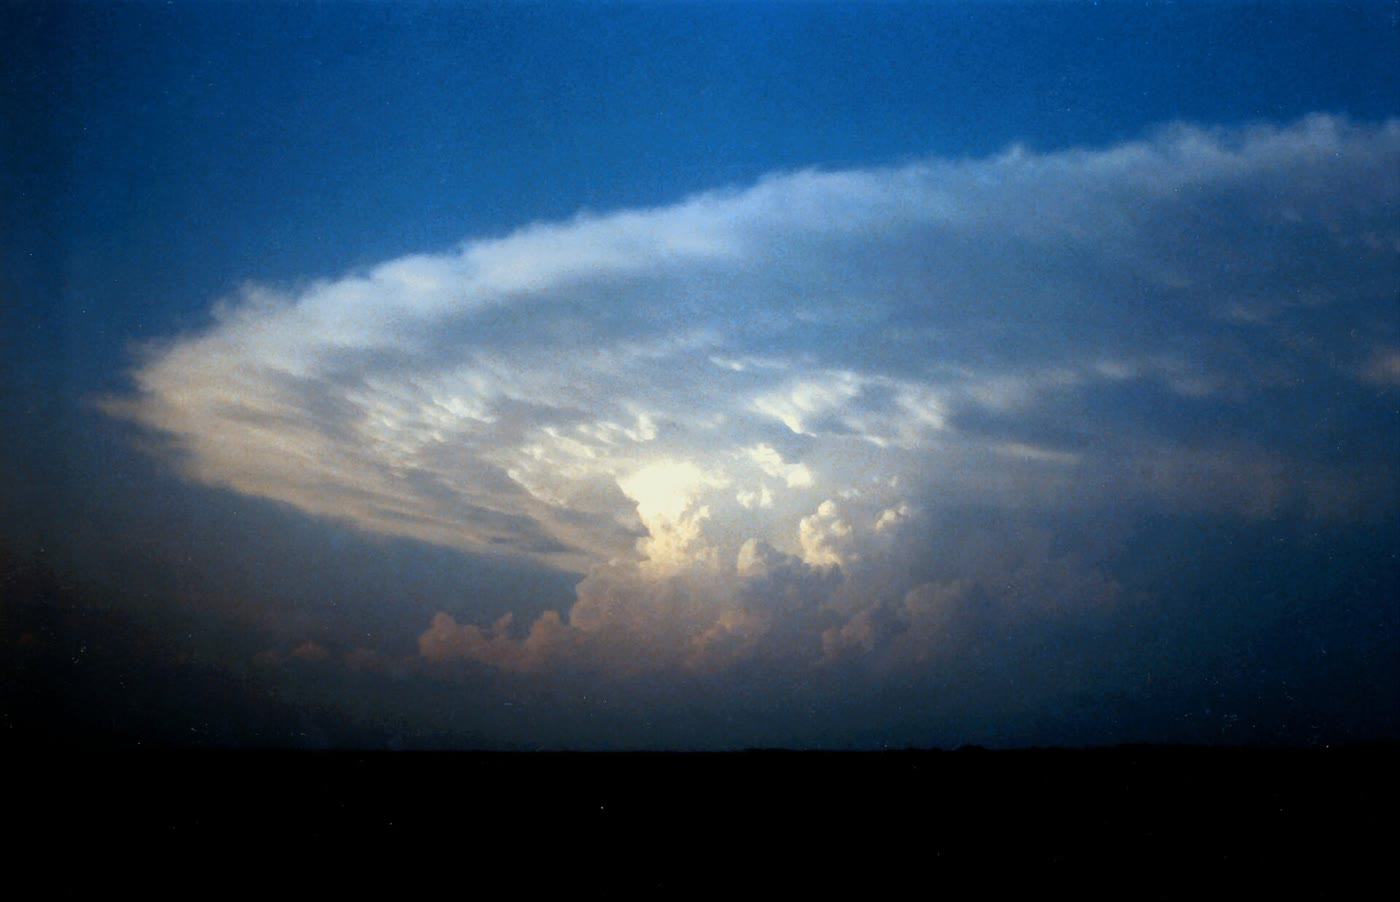
\includegraphics[width=0.6\linewidth]{images/book4/b2-21-supercell-anvil.jpg}
\par\smallskip{\small Un orage au-dessus du Nebraska, le 20 avril 1985~: son courant ascendant s'étale en
enclume là où il atteint son \omterm{def:b2:atmospheric-thermodynamics:parcel-levels}{niveau d'équilibre}, près de la tropopause. (Stephen Corfidi,
NOAA/NWS, domaine public, via Wikimedia Commons.)}
\end{omfigure}
% ledger: nws4:lfc-el

\section{Microphysique des nuages}\label{sec:b2:atmospheric-thermodynamics:microphysics}

Une particule d'air à son LCL est saturée au-dessus d'une surface d'eau plane. Une gouttelette n'est pas plane~:
les volumes de physique montrent qu'une nouvelle phase n'apparaît pas à l'équilibre, mais seulement par
germination, et les volumes de chimie que la \omterm{def:b2:atmospheric-thermodynamics:moist-air}{pression de vapeur} au-dessus d'une surface courbe dépasse celle
au-dessus d'une surface plane (l'équation de Kelvin). Avec la constante $A$ de la \cref{prop:b2:atmospheric-thermodynamics:kohler}
ci-dessous, une gouttelette d'eau pure de \qty{2}{nm} de diamètre n'est en équilibre qu'au
rapport de saturation $\exp(2.1/2) = 2.9$, soit une \omterm{def:b2:atmospheric-thermodynamics:microphysics}{sursaturation} de \qty{190}{\percent}, bien au-dessus des
fractions de pour cent auxquelles les particules s'activent~: les gouttelettes se forment sur des particules.

\begin{definition}[Sursaturation~; noyau de condensation nuageuse]\label{def:b2:atmospheric-thermodynamics:microphysics}
La \emph{sursaturation}\index{sursaturation} de l'air est $s = e/e_s - 1$, l'excès de sa \omterm{def:b2:atmospheric-thermodynamics:moist-air}{pression de
vapeur} sur la \omterm{def:b2:atmospheric-thermodynamics:moist-air}{pression de vapeur} saturante au-dessus d'une surface plane d'eau pure, souvent exprimé
en pour cent. Un \emph{noyau de condensation nuageuse}\index{noyau de condensation nuageuse} (CCN) est
une particule d'aérosol sur laquelle une gouttelette de nuage se forme aux faibles sursaturations
des nuages. C'est le \emph{noyau de condensation}\index{noyau de condensation} des volumes scolaires.
\end{definition}
% ledger: nws4:ccn-bergeron, pk07:kohler, morrison20:processes

\begin{proposition}[Courbe de Köhler]\label{prop:b2:atmospheric-thermodynamics:kohler}
\index{courbe de Köhler}
Une gouttelette de solution de diamètre $D$, formée sur une particule sèche de diamètre
$D_d$ et d'hygroscopicité $\kappa$, est en équilibre avec le rapport de saturation
\[
  S(D) = \frac{D^3 - D_d^3}{D^3 - D_d^3(1 - \kappa)}\,\exp\Bigl(\frac{A}{D}\Bigr), \qquad
  A = \frac{4\sigma M_w}{R T\rho_w},
\]
avec $\sigma$ la tension superficielle et $\rho_w$ la masse volumique de l'eau
(admise). La courbe $S(D)$ est la \emph{\omterm{prop:b2:atmospheric-thermodynamics:kohler}{courbe de Köhler}}. Pour $D \gg D_d$,
\[
  s = S - 1 \approx \frac{A}{D} - \frac{\kappa D_d^3}{D^3},
\]
qui est maximale au diamètre et à la \omterm{def:b2:atmospheric-thermodynamics:microphysics}{sursaturation} critiques~:
\[
  D_c = \sqrt{\frac{3\kappa D_d^3}{A}}, \qquad s_c = \sqrt{\frac{4A^3}{27\,\kappa D_d^3}} .
\]
\end{proposition}
% ledger: pk07:kohler

\begin{proof}[Démonstration de l'approximation]
L'exponentielle est le facteur de Kelvin~; la fraction est l'activité de l'eau, une version de
la loi de Raoult où $\kappa$ mesure la quantité d'eau que retient la matière dissoute. Pour
$D \gg D_d$ et $A \ll D$, $\exp(A/D) \approx 1 + A/D$ et la fraction vaut $1 - \kappa D_d^3/D^3$ au
premier ordre~; le produit, au premier ordre, est $1 + A/D - \kappa D_d^3/D^3$. En annulant la
dérivée $-A/D^2 + 3\kappa D_d^3/D^4$, on obtient $D_c^2 = 3\kappa D_d^3/A$, puis $s_c = A/D_c -
A/(3D_c) = 2A/(3D_c)$, ce qui est la formule.
\end{proof}

Avec $\sigma = \qty{0.072}{J/m^2}$ à \qty{298.15}{K}, $A = \qty{2.1}{nm}$. Le sulfate d'ammonium a $\kappa = 0.61$~; le
chlorure de sodium est encore plus hygroscopique ($\kappa = 1.28$), et les particules atmosphériques se situent surtout
entre 0.1 et 0.9. Une particule sèche de \qty{50}{nm} de sulfate d'ammonium a $D_c = \qty{0.33}{\micro m}$ et $s_c =
\qty{0.42}{\percent}$~; une de \qty{100}{nm}, \qty{0.93}{\micro m} et \qty{0.15}{\percent}.
L'approximation diffère du maximum exact de moins de \qty{1}{\percent}.
% ledger: pk07:kohler, pk07:kappa

\begin{omfigure}
\centering
% figdata/bachelor-2/thermo.py part kohler
\begin{tikzpicture}
\begin{semilogxaxis}[width=0.72\linewidth, height=5.6cm, xmin=0.03, xmax=10, ymin=-0.4,
  ymax=1.1, xlabel={diamètre de la gouttelette $D$ (\unit{\micro m})}, ylabel={sursaturation $s$
  (\unit{\percent})}, tick label style={font=\scriptsize}, label style={font=\small},
  log ticks with fixed point, legend style={font=\scriptsize, draw=none, fill=none},
  legend pos=north east, legend cell align=left, unbounded coords=discard]
\addplot[ocBlue, thick, densely dotted] table[x=D_um, y=s30] {figdata/out/bachelor-2-thermo-kohler.dat};
\addlegendentry{$D_d = \qty{30}{nm}$}
\addplot[ocBlue, thick] table[x=D_um, y=s50] {figdata/out/bachelor-2-thermo-kohler.dat};
\addlegendentry{$D_d = \qty{50}{nm}$}
\addplot[ocBlue, thick, dashed] table[x=D_um, y=s100] {figdata/out/bachelor-2-thermo-kohler.dat};
\addlegendentry{$D_d = \qty{100}{nm}$}
\addplot[only marks, mark=*, mark size=1.5pt, black] coordinates {(0.1542,0.914) (0.3309,0.4244)
  (0.9345,0.1499)};
\draw[black!45] (axis cs:0.03,0) -- (axis cs:10,0);
\draw[ocRed, densely dashed] (axis cs:0.03,0.5) -- (axis cs:10,0.5);
\node[font=\scriptsize, ocRed, anchor=north west] at (axis cs:2.2,0.5) {$s = \qty{0.5}{\percent}$};
\end{semilogxaxis}
\end{tikzpicture}
\par\smallskip{\small \omterm{prop:b2:atmospheric-thermodynamics:kohler}{Courbes de Köhler} de particules de sulfate d'ammonium ($\kappa = 0.61$) de trois diamètres
secs, à \qty{298.15}{K}, avec leurs points critiques (marqués d'un point). Dans un air à
\qty{0.5}{\percent} de \omterm{def:b2:atmospheric-thermodynamics:microphysics}{sursaturation}, les particules de \qty{50}{nm} et de \qty{100}{nm} grandissent sans
limite~; la particule de \qty{30}{nm} reste une gouttelette de brume.}
\end{omfigure}
% ledger: pk07:kohler, pk07:kappa

La courbe partage les particules. Sous son sommet, une gouttelette est en équilibre stable~: si elle grossit,
l'air n'est plus assez sursaturé pour elle et elle rétrécit~; de telles gouttelettes de brume gonflent et
rétrécissent avec l'humidité. Dès que la \omterm{def:b2:atmospheric-thermodynamics:microphysics}{sursaturation} de l'air dépasse $s_c$, la gouttelette est \emph{activée}~:
au-delà du sommet, elle a besoin de moins en moins de \omterm{def:b2:atmospheric-thermodynamics:microphysics}{sursaturation} à mesure qu'elle grossit, et elle grossit
tant qu'il y a de la vapeur. Une particule qui monte se refroidit, sa \omterm{def:b2:atmospheric-thermodynamics:microphysics}{sursaturation} augmente, et les particules
les plus grosses et les plus solubles s'activent les premières~; les gouttelettes qu'elles forment prennent
alors la vapeur et plafonnent la \omterm{def:b2:atmospheric-thermodynamics:microphysics}{sursaturation}. Au-dessus des océans lointains, il y a environ 110 CCN par centimètre
cube actives à \qty{0.4}{\percent}, au-dessus des continents lointains presque deux fois plus, et dans un
air pollué environ dix fois plus. La même eau partagée entre davantage de gouttelettes les rend plus petites.
% ledger: andreae09:ccn, morrison20:processes

\begin{remark}[Pourquoi la condensation seule ne fait pas la pluie]\label{rem:b2:atmospheric-thermodynamics:growth}
Une gouttelette grossit par diffusion de la vapeur vers elle. Le flux à travers une sphère entourant une
gouttelette de rayon $r$ vaut $4\pi r D_v\,\Delta\rho_v$, avec $D_v$ la diffusivité de la vapeur et $\Delta\rho_v$
l'excès de masse volumique de vapeur loin d'elle, de sorte que sa masse $\tfrac43\pi r^3\rho_w$ croît à un
taux proportionnel à $r$~: $r\,\mathrm{d}r/\mathrm{d}t$ est constant et $r^2$ croît linéairement en fonction
du temps. Les grosses gouttelettes grossissent plus lentement que les petites, et une population qui croît
par condensation seule devient plus étroite, non plus large. Les gouttes de pluie se forment lorsque des
gouttelettes de tailles différentes, qui tombent à des vitesses différentes, entrent en collision et coalescent.
\end{remark}
% ledger: morrison20:processes

Au-dessus du niveau où la température vaut \qty{0}{\celsius}, un nuage est fait de gouttelettes en
surfusion jusqu'à ce que des particules glaciogènes amorcent des cristaux de glace. Alors agit la
différence du panneau de droite de la figure de saturation~: l'air saturé au-dessus des gouttelettes est
sursaturé de \qty{10}{\percent} par rapport à la glace à \qty{-10}{\celsius}, soit des dizaines de
fois les \omterm{def:b2:atmospheric-thermodynamics:microphysics}{sursaturations} auxquelles les gouttelettes se sont activées. Les cristaux grandissent par
dépôt aux dépens des gouttelettes, qui s'évaporent (le processus de Bergeron, le processus des
cristaux de glace des volumes scolaires), et ils captent les gouttelettes qui gèlent sur eux (givrage).
% ledger: nws4:ccn-bergeron, morrison20:processes, iapws4:sublimation

\begin{omfigure}
\centering
\begin{tikzpicture}[font=\scriptsize, box/.style={draw=black!60, rounded corners=2pt,
  align=center, minimum height=0.95cm, text width=2.1cm, fill=#1}, box/.default=white,
  >=Stealth]
\node[anchor=west, black!60] at (-1.15,0.8) {processus chauds};
\node[box=black!6] (ccn) at (0,0) {particule d'aérosol\\(CCN)};
\node[box=ocBlue!8] (haze) at (4.2,0) {gouttelette de brume\\$s < s_c$};
\node[box=ocBlue!15] (act) at (8.4,0) {gouttelette activée\\$s > s_c$};
\node[box=ocBlue!25] (rain) at (12.6,0) {goutte de pluie};
\draw[->] (ccn) -- node[above] {humidité} (haze);
\draw[->] (haze) -- node[above] {ascendance} (act);
\draw[->] (act) -- node[above, align=center] {collision,\\coalescence} (rain);
\node[anchor=west, black!60] at (-1.15,-3.4) {processus glaciaires};
\node[box=black!6] (inp) at (0,-2.6) {particule\\glaçogène};
\node[box=omMeth!10] (ice) at (4.2,-2.6) {cristal de glace\\sous \qty{0}{\celsius}};
\node[box=omMeth!20] (snow) at (8.4,-2.6) {neige, grésil};
\node[box=ocBlue!25] (rain2) at (12.6,-2.6) {pluie};
\draw[->] (inp) -- (ice);
\draw[->] (ice) -- node[above, align=center] {dépôt,\\givrage} (snow);
\draw[->] (snow) -- node[above] {fonte} (rain2);
\draw[->, omMeth!60!black, dashed] (act.south) -- node[pos=0.45, right=4pt, align=left,
  omMeth!60!black] {vapeur issue des\\gouttelettes qui s'évaporent} (ice.north);
\end{tikzpicture}
\par\smallskip{\small Les deux chemins de la vapeur vers les précipitations~: activation et croissance des gouttelettes,
puis collision et coalescence (en haut)~; cristaux de glace qui grandissent aux dépens des gouttelettes en surfusion,
givrent, et fondent en tombant dans un air plus chaud (en bas).}
\end{omfigure}
% ledger: morrison20:processes, nws4:ccn-bergeron

\begin{inthefield}[Un lancer du matin]
\begin{minipage}[t]{0.54\linewidth}\vspace{0pt}
À chaque station de \omterm{def:b2:atmospheric-thermodynamics:sounding}{radiosondage}, le technicien prépare le ballon et la radiosonde dans l'heure qui
précède 00 et 12~UTC, les heures auxquelles plus de huit cents stations du monde observent
ensemble. L'instrument, de 60 à \qty{80}{g}, pend sous le ballon et transmet la pression, la température,
l'humidité et sa position par satellite chaque seconde. Le ballon monte d'environ \qty{300}{m}
par minute, pendant deux heures ou plus, au-delà de \qty{35}{km} avant d'éclater, et peut dériver
de plus de \qty{300}{km}. Les prévisionnistes tracent le profil sur un \omterm{def:b2:atmospheric-thermodynamics:diagram}{émagramme oblique}, et
les jours où un temps violent est attendu, certaines stations lâchent des ballons supplémentaires.
\end{minipage}\hfill
\begin{minipage}[t]{0.42\linewidth}\vspace{0pt}
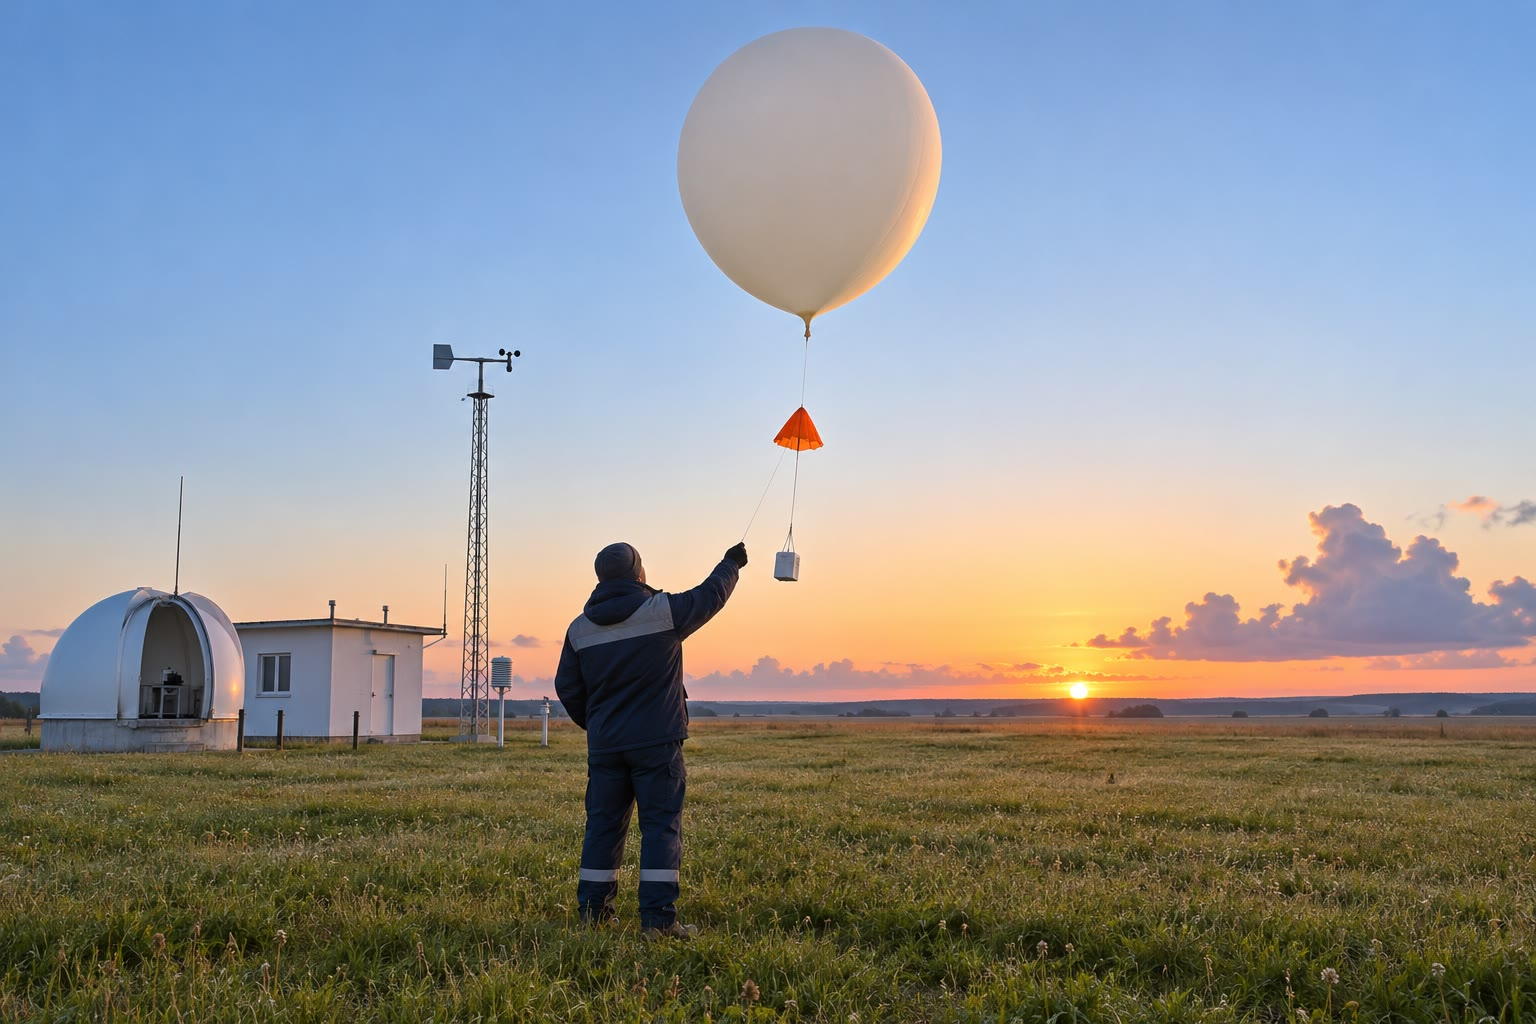
\includegraphics[width=\linewidth]{images/book4/ai/b2-radiosonde-launch.jpg}

{\scriptsize Une radiosonde lâchée à l'aube depuis une station météorologique (Illustration
générée par IA.)}
\end{minipage}
% ledger: nws:radiosonde, nws4:upperair
\end{inthefield}

\section*{Exercices}\label{sec:b2:atmospheric-thermodynamics:exercises}

Données des exercices, sauf indication contraire~: $e_s(T) = \qty{6.117}{hPa} \times
\exp[\qty{5419}{K} \times (1/\qty{273.16}{K} - 1/T)]$~; $\varepsilon = 0.622$, $R_d =
\qty{287.0}{J.kg^{-1}.K^{-1}}$, $R_v = \qty{461.5}{J.kg^{-1}.K^{-1}}$, $c_p =
\qty{1004.5}{J.kg^{-1}.K^{-1}}$, $L = \qty{2.501e6}{J/kg}$,
$g = \qty{9.81}{m.s^{-2}}$, $\Gamma_d = \qty{9.8}{K/km}$.
% ledger: nist4:water-sat, iapws4:sublimation, const:R, earth:Mmol, nist4:water-mw, nasa:grc-gamma

\begin{exercise}[$\star$]\label{exo:b2:atmospheric-thermodynamics:1}
À \qty{850}{hPa}, la température est de \qty{10.0}{\celsius} et le point de rosée de \qty{5.0}{\celsius}.
(a) Calculer la \omterm{def:b2:atmospheric-thermodynamics:moist-air}{pression de vapeur} et la \omterm{def:b2:atmospheric-thermodynamics:moist-air}{pression de vapeur} saturante. (b) Calculer l'humidité
relative. (c) Calculer le \omterm{def:b2:atmospheric-thermodynamics:moist-air}{rapport de mélange} et l'\omterm{def:b2:atmospheric-thermodynamics:moist-air}{humidité spécifique}, en grammes par kilogramme.
\end{exercise}

\begin{exercise}[$\star$]\label{exo:b2:atmospheric-thermodynamics:2}
(a) De combien de pour cent par kelvin $e_s$ augmente-t-elle à \qty{0}{\celsius}, \qty{20}{\celsius}
et \qty{30}{\celsius}~? (b) Calculer $e_s$ à \qty{20}{\celsius} et à \qty{25}{\celsius},
ainsi que leur rapport~; le comparer à $1.063^5$. (c) La valeur mesurée à \qty{20}{\celsius}
est \qty{23.39}{hPa}. De combien la formule se trompe-t-elle, et dans quel sens~? Pourquoi~?
\end{exercise}
% ledger: nist4:water-sat

\begin{exercise}[$\star$]\label{exo:b2:atmospheric-thermodynamics:3}
À midi, l'air de surface est à \qty{30}{\celsius} avec un point de rosée de \qty{14}{\celsius}. (a) Calculer à
quelle hauteur au-dessus du sol se forment les bases des cumulus. (b) Calculer la température d'une particule à
ce niveau, par l'adiabatique sèche. (c) Calculer son point de rosée à ce niveau, avec $\Gamma_{\text{rosée}} =
\qty{1.8}{K/km}$. Commenter. (d) Plus tard, l'air se réchauffe jusqu'à \qty{33}{\celsius},
le point de rosée restant inchangé. Où se trouvent maintenant les bases des nuages~?
\end{exercise}

\begin{exercise}[$\star$]\label{exo:b2:atmospheric-thermodynamics:4}
Lire l'\omterm{def:b2:atmospheric-thermodynamics:diagram}{émagramme oblique} du \omterm{def:b2:atmospheric-thermodynamics:sounding}{radiosondage} de Norman. (a) Jusqu'à quelle pression l'air proche du
sol est-il saturé, ou presque~? (b) Où se trouve l'inversion, et comment se manifeste-t-elle~? (c)
Lire le LCL, le LFC et l'EL de la particule de surface. (d) Comment le point de rosée et la
température se comparent-ils juste au-dessus de l'inversion, et qu'est-ce que cela dit de cet air~?
\end{exercise}
% ledger: data:b4-sounding

\begin{exercise}[$\star\star$]\label{exo:b2:atmospheric-thermodynamics:5}
De l'air tropical à \qty{1000}{hPa} a $T = \qty{30.0}{\celsius}$ et $r = \qty{20}{g/kg}$. (a) Calculer sa
\omterm{def:b2:atmospheric-thermodynamics:virtual}{température virtuelle} exactement, puis avec l'approximation $T(1 + 0.61\,r)$. (b) Calculer les masses volumiques
de cet air et de l'air sec à même température et même pression. (c) De combien faudrait-il réchauffer l'air sec
pour qu'il soit aussi léger~? (d) Pourquoi cela compte-t-il pour la convection au-dessus des mers chaudes~?
\end{exercise}

\begin{exercise}[$\star\star$]\label{exo:b2:atmospheric-thermodynamics:6}
Utiliser la \cref{prop:b2:atmospheric-thermodynamics:gamma-s} à \qty{1000}{hPa}, avec $r_s$
tiré de la \cref{prop:b2:atmospheric-thermodynamics:humidity}. (a) Calculer $r_s$ et $\Gamma_s$
à \qty{0}{\celsius}, \qty{20}{\celsius} et \qty{30}{\celsius}. (b) Si son gradient reste le
même, de combien une particule saturée à \qty{20}{\celsius} est-elle plus chaude qu'une
particule sèche après une montée de \qty{1}{km}~? (c) Pourquoi l'écart diminue-t-il plus haut~?
\end{exercise}

\begin{exercise}[$\star\star$]\label{exo:b2:atmospheric-thermodynamics:7}
La particule de surface de Norman ($p = \qty{971.1}{hPa}$, $T = \qty{19.0}{\celsius}$, $T_d =
\qty{18.5}{\celsius}$) a son LCL à la température de \qty{18.35}{\celsius}. (a) Calculer
son \omterm{def:b2:atmospheric-thermodynamics:moist-air}{rapport de mélange}, sa température potentielle et sa \omterm{def:b2:atmospheric-thermodynamics:theta-e}{température potentielle équivalente}.
(b) Soulevée, elle se trouve à \qty{-8.9}{\celsius} à \qty{500}{hPa}, saturée.
Calculer son $\theta$ et son $\theta_e$ à ce niveau. (c) Laquelle des deux est conservée~?
\end{exercise}
% ledger: data:b4-sounding

\begin{exercise}[$\star\star$]\label{exo:b2:atmospheric-thermodynamics:8}
Une particule est plus chaude que son environnement de \qty{4}{K} entre \qty{700}{hPa}, son LFC,
et \qty{300}{hPa}, son EL~; négliger la correction de \omterm{def:b2:atmospheric-thermodynamics:virtual}{température virtuelle}. (a) Calculer sa
CAPE. (b) Calculer $w_{\max}$. (c) Dans quelle classe tombe la CAPE~? (d) Sur un \omterm{def:b2:atmospheric-thermodynamics:diagram}{émagramme
oblique}, quelle forme a l'aire positive, et pourquoi son aire est-elle celle qui a été calculée~?
\end{exercise}
% ledger: hgx:cape

\begin{exercise}[$\star\star$]\label{exo:b2:atmospheric-thermodynamics:9}
Prendre $A = \qty{2.1}{nm}$ et le sulfate d'ammonium, $\kappa = 0.61$. (a) Calculer le diamètre
critique et la \omterm{def:b2:atmospheric-thermodynamics:microphysics}{sursaturation} critique d'une particule sèche de \qty{80}{nm}. (b) Quelle est la plus
petite particule sèche activée dans un air à \qty{0.3}{\percent} de \omterm{def:b2:atmospheric-thermodynamics:microphysics}{sursaturation}~? À
\qty{0.1}{\percent}~? (c) Un courant ascendant fait passer la \omterm{def:b2:atmospheric-thermodynamics:microphysics}{sursaturation} de \qty{0.1}{\percent} à
\qty{0.3}{\percent}~: que devient le nombre de gouttelettes, et leur taille pour la même eau liquide~?
\end{exercise}
% ledger: pk07:kappa, pk07:kohler

\begin{exercise}[$\star\star\star$]\label{exo:b2:atmospheric-thermodynamics:10}
La particule de surface de Norman avait une CIN d'environ \qty{-130}{J/kg} avec la \omterm{def:b2:atmospheric-thermodynamics:virtual}{température
virtuelle}. (a) À quelle vitesse verticale devrait-elle quitter le sol pour atteindre son
LFC par son seul élan~? (b) Le sommet de l'inversion est à \qty{889.1}{hPa} et \qty{20.5}{\celsius}.
À quelle température l'air de surface à \qty{971.1}{hPa} doit-il se réchauffer pour
qu'une particule soulevée de façon adiabatique sèche ne soit pas plus froide que le sommet de
l'inversion~? (c) Si son point de rosée restait à \qty{18.5}{\celsius}, où serait sa base
de nuage~? (d) Citer deux façons dont l'atmosphère supprime un tel couvercle sans le soleil.
\end{exercise}
% ledger: data:b4-sounding, nws4:cin

\begin{exercise}[$\star\star\star$]\label{exo:b2:atmospheric-thermodynamics:11}
(a) Montrer à partir de la \cref{prop:b2:atmospheric-thermodynamics:gamma-s} que $\Gamma_s \to \Gamma_d$
lorsque $r_s \to 0$. (b) Montrer que, lorsque $Lr_s/(R_dT) \gg 1$, $\Gamma_s \to gR_vT/(LR_d)$,
et l'évaluer à \qty{303}{K}. (c) Comparer avec $\Gamma_{\text{rosée}}$ de la
\cref{prop:b2:atmospheric-thermodynamics:lcl} lorsque $T_d = T$, et expliquer pourquoi les deux limites
coïncident. (d) La limite de (b) est-elle atteinte dans l'atmosphère~? Utiliser la valeur $\Gamma_s =
\qty{3.4}{K/km}$ à \qty{30}{\celsius} et \qty{1000}{hPa}.
\end{exercise}

\begin{exercise}[$\star\star\star$]\label{exo:b2:atmospheric-thermodynamics:12}
Au-dessus de l'eau en surfusion et au-dessus de la glace, les \omterm{def:b2:atmospheric-thermodynamics:moist-air}{pressions de vapeur} saturante valent
2.868 et \qty{2.599}{hPa} à \qty{-10}{\celsius}, 1.257 et \qty{1.032}{hPa} à \qty{-20}{\celsius}.
(a) Calculer la \omterm{def:b2:atmospheric-thermodynamics:microphysics}{sursaturation} par rapport à la glace de l'air saturé par rapport à l'eau, aux
deux températures. (b) Comparer avec les \omterm{def:b2:atmospheric-thermodynamics:microphysics}{sursaturations} auxquelles les gouttelettes s'activent.
(c) Expliquer pourquoi un nuage de gouttelettes en surfusion qui reçoit quelques cristaux de
glace se transforme en glace. (d) Pourquoi l'effet est-il plus faible près de \qty{0}{\celsius}~?
\end{exercise}
% ledger: iapws4:sublimation, su26:svp, nws4:ccn-bergeron

\begin{problem}[{Problème du week-end --- Lire le radiosondage du matin}]\label{pb:b2:atmospheric-thermodynamics:1}
Le tableau donne le \omterm{def:b2:atmospheric-thermodynamics:sounding}{radiosondage} de 12~UTC à Norman, Oklahoma, le 16 avril 2026, aux niveaux utilisés
ici~: pression, altitude au-dessus du niveau de la mer, température, point de rosée, et
température de la particule de surface soulevée comme dans la \cref{met:b2:atmospheric-thermodynamics:lift},
calculée en intégrant la \cref{prop:b2:atmospheric-thermodynamics:gamma-s} par petits pas.
Le \omterm{def:b2:atmospheric-thermodynamics:sounding}{radiosondage} situe la tropopause à \qty{235.3}{hPa} et \qty{10954}{m}. Utiliser les données
des exercices et les températures (et non les \omterm{def:b2:atmospheric-thermodynamics:virtual}{températures virtuelles}), sauf indication contraire.

\begin{center}
\small
\begin{tabular}{rrrrr}
\hline
$p$ (\unit{hPa}) & $z$ (\unit{m}) & $T$ (\unit{\celsius}) & $T_d$ (\unit{\celsius}) &
$T_{\text{particule}}$ (\unit{\celsius}) \\
\hline
971.1 & 345 & 19.0 & 18.5 & 19.0 \\
925.0 & 763 & 17.3 & 17.3 & 16.9 \\
907.7 & 924 & 16.4 & 16.4 & 16.2 \\
889.1 & 1102 & 20.5 & 9.5 & 15.4 \\
850.0 & 1489 & 18.6 & $-1.8$ & 13.7 \\
700.0 & 3110 & 4.5 & $-12.2$ & 6.1 \\
500.0 & 5725 & $-18.4$ & $-36.6$ & $-8.9$ \\
400.0 & 7357 & $-30.4$ & $-55.6$ & $-20.4$ \\
300.0 & 9349 & $-42.7$ & $-66.3$ & $-37.1$ \\
250.0 & 10560 & $-49.8$ & $-69.8$ & $-48.3$ \\
200.0 & 12006 & $-52.3$ & $-78.3$ & $-61.8$ \\
\hline
\end{tabular}
\end{center}

\medskip\noindent\textbf{Partie I --- L'air près du sol.}
\begin{enumerate}
  \item Calculer la \omterm{def:b2:atmospheric-thermodynamics:moist-air}{pression de vapeur} de l'air de surface, à une décimale près.
  \item Calculer son \omterm{def:b2:atmospheric-thermodynamics:moist-air}{rapport de mélange}, à une décimale près.
  \item Calculer son \omterm{def:b2:atmospheric-thermodynamics:moist-air}{humidité spécifique}.
  \item Calculer son humidité relative.
  \item De combien sa \omterm{def:b2:atmospheric-thermodynamics:virtual}{température virtuelle} dépasse-t-elle sa température~?
  \item Calculer la hauteur de son LCL au-dessus du sol avec la règle de \qty{125}{m} par degré, ainsi que la pression
        à ce niveau (prendre une \omterm{def:b2:atmospheric-thermodynamics:virtual}{température virtuelle} moyenne de \qty{294.7}{K} pour la couche).
  \item Calculer sa température potentielle.
\end{enumerate}

\medskip\noindent\textbf{Partie II --- Le couvercle et les couches au-dessus.}
\begin{enumerate}[resume]
  \item À \qty{925}{hPa}, la particule est-elle plus chaude ou plus froide que son environnement, et de combien~?
  \item Calculer le gradient vertical entre 907.7 et \qty{889.1}{hPa}. De quel type de couche s'agit-il~?
  \item De combien la particule est-elle plus froide que son environnement à \qty{889.1}{hPa}~?
  \item Calculer l'humidité relative à \qty{850}{hPa}. D'où un tel air a-t-il pu venir~?
  \item Calculer le gradient vertical moyen entre 850 et \qty{500}{hPa} et classer la couche.
  \item Calculer l'indice de soulèvement et sa classe.
\end{enumerate}

\medskip\noindent\textbf{Partie III --- L'énergie.}
\begin{enumerate}[resume]
  \item Calculer l'écart $\Delta T = T_{\text{particule}} - T$ à chaque niveau du tableau.
  \item Calculer le LFC par interpolation linéaire de $\Delta T$ en $\ln p$, à l'hectopascal près,
        et son altitude par interpolation de $z$ de la même façon.
  \item Calculer l'EL et son altitude de la même façon. Comparer avec la tropopause.
  \item Calculer la CAPE par la méthode des trapèzes en $\ln p$, du LFC à l'EL en passant par les
        niveaux du tableau.
  \item Dans quelle classe tombe-t-elle~?
  \item Calculer la CIN de la même façon, du sol jusqu'au LFC.
  \item Un calcul sur une grille de \qty{1}{hPa} donne une CAPE de \qty{2100}{J/kg} avec les
        températures et \qty{2230}{J/kg} avec les \omterm{def:b2:atmospheric-thermodynamics:virtual}{températures virtuelles}. Pourquoi les trois valeurs
        diffèrent-elles~?
\end{enumerate}

\medskip\noindent\textbf{Partie IV --- L'orage que l'air pouvait alimenter.}
\begin{enumerate}[resume]
  \item Quelle vitesse verticale la théorie de la particule donne-t-elle avec la CAPE de la question 17~?
  \item À la moitié de cette vitesse tout au long de la montée, combien de temps l'air mettrait-il pour monter du LFC à l'EL~?
  \item Citer deux effets qui ralentissent un courant ascendant réel.
  \item En résumé, quelle vitesse de courant ascendant la théorie de la particule prévoit-elle
        pour un orage alimenté par l'air de surface de ce matin~?
\end{enumerate}
\end{problem}
% ledger: data:b4-sounding, hgx:cape, nws4:lifted-index, nws4:cape
